\input{header}

\AtBeginSubsection[]
{
	\begin{frame}<beamer>
		\frametitle{Outline}
		\tableofcontents[current,currentsubsection]
	\end{frame}
}

\begin{document}

\begin{frame}[allowframebreaks] \frametitle{Polynomial vs. Exponential}
  \begin{itemize}
\item Big difference
\item $n^3: n = 1000 \Rightarrow 10^9$
\item $2^n: n = 1000 \Rightarrow 2^{1000}
=10^{1000\log_{10}2}
\approx
10^{300}
\gg 10^9$

\item An algorithm with such complexity is not practical
\end{itemize}\end{frame}

\begin{frame}[allowframebreaks] \frametitle{Definition 7.2}
  \begin{itemize}
\item $P$: decidable languages in polynomial time
on a deterministic (single-tape) TM
\begin{equation*}
  P=\cup_k
\text{TIME}(n^k).
\end{equation*}
\item How important this is ?

\item [] $P$: ``roughly'' corresponds to problems solvable
on a computer

% \end{itemize}\end{frame} \begin{frame}[allowframebreaks] \frametitle{Examples of P}
% \item Description on pages 236 and 237

% not very important

\end{itemize}\end{frame} \begin{frame}[allowframebreaks] \frametitle{PATH problem}
\begin{eqnarray*}
&&  \text{PATH}
=\{
\langle  G,s,t\rangle \mid \mbox{$G$ is a directed graph}\\
&& \qquad\qquad\qquad
\mbox{such that $\exists$ path from $s$ to $t$}\}
\}
\end{eqnarray*}
  \begin{itemize}
  \item Example:

  \begin{center}
    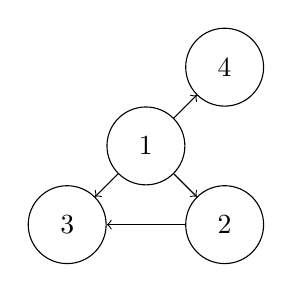
\begin{tikzpicture}
[inner sep=2.5mm]      
\path ( 0,0) node (3) [shape=circle,draw] {3}
( 2,0) node (2) [shape=circle,draw] {2}
( 2,2) node (4) [shape=circle,draw] {4}
( 1,1) node (1) [shape=circle,draw] {1};
\draw [->] (1) -- (2);
\draw [->] (2) -- (3);
\draw [->] (1) -- (3);
\draw [->] (1) -- (4);
\end{tikzpicture}
\end{center}
\item[] There is a path from $s=1$ to $t=3$
\item We will prove that PATH $\in P$
\item Let's start with a brute force way

  \begin{enumerate}
  \item $m$: \# nodes

  \item $|\text{path}|\leq m$

  \item \#paths $\leq m^m$

  \item sequentially check if one has $s$ to $t$

  \end{enumerate}
  \item the cost is exponential  
\item A polynomial algorithm

\item [] input $\langle  G,s,t\rangle $, $G$ includes nodes and edges
\begin{enumerate}
\item mark $s$


\item repeat until no new node can be marked

  \quad scan all edges, if for an edge $\langle  a,b\rangle $:
  \begin{center}
  $a$ is marked but $b$ is not
$\Rightarrow $ mark $b$
\end{center}
\item $t$ marked $\Rightarrow$ accept

otherwise $\Rightarrow$ reject
\end{enumerate}
\item \# of steps in the main loop: at most $m$ (if no newly marked, stop)
\item at each step, need to scan \#edges$\leq m^2$
\item cost to mark a node: polynomial
\item whole algorithm: polynomial
\end{itemize}\end{frame} \begin{frame}[allowframebreaks] \frametitle{Relatively Prime}
  \begin{itemize}
\item $x,y$ are relatively prime if they have no common ($> 1$) factors

\item Example: 10 and 21
  \begin{equation*}
10=2 \times 5, 21
=3\times 7
\end{equation*}
\item Example: 10 and 22
  \begin{equation*}
10=2 \times 5, 22
=2\times 11
\end{equation*}
They are not relatively prime
\item Problem: test if two numbers are relatively
prime
\end{itemize}\end{frame} \begin{frame}[allowframebreaks] \frametitle{Euclidean Algorithm}
  \begin{itemize}
\item It can be used to find gcd (greatest common divisor)
\item Example:  gcd(18,24)=6
\item We have
  \begin{center}
gcd($x,y$)=1
$\Leftrightarrow$ $x,y$ relatively prime
\end{center}
\item Algorithm: input $\langle  x,y\rangle $
  \begin{enumerate}
  \item Repeat if $y \neq 0$
    \begin{equation*}
x \leftarrow x \text{ mod } y
\end{equation*}
exchange $x$ and $y$
\item Output $x$
  \end{enumerate}
\item The output is the gcd
\item Note that in the beginning we don't need
  \begin{equation*}
    x\geq y
  \end{equation*}
If
\begin{equation*}
  x < y,
\end{equation*}
then
\begin{equation*}
  x = x \text{ mod } y
\end{equation*}
and
\begin{equation*}
  (x,y) \text{ becomes } (y,x)
\end{equation*}
\item Why this works
  \begin{equation*}
    \begin{split}
& 18=ab \\
& 24=ac \\
& 24 = 18d + e \\
& ac=abd + e \\
& e = a (c-bd) \\
& a \mid  24-18d
\end{split}
\end{equation*}
\item Is this algorithm polynomial?

\item At each iteration, $x$ or $y$ reduced at least by half 
  
\item If $x > y$
\begin{equation*}
  x \text{ mod } y \leq x/2
\end{equation*}
Proof
\begin{equation*}
  \mbox{if } x/2 \geq y, x \text{ mod } y \leq y \leq x/2
\end{equation*}
\begin{equation*}
  \mbox{if } x/2 < y, x \text{ mod } y = x-y \leq x/2
\end{equation*}
\item Therefore,
  \begin{equation*}
\text{\#iterations } \leq 2\max(\log_2 x, \log_2 y)= O(n)
\end{equation*}
$n$: length of input ($x$ and $y$ are stored as bit strings), $\log_2 x + \log_2 y$
\item Each iteration

\item [] $x \text{ mod } y$:  polynomial

\item [] see: 1100011 \% 101

\item [] \#digit $\leq O(n)$: each digit $\leq O(n)$

\item [] exchange $x$ and $y$: polynomial

\end{itemize}\end{frame}

\begin{frame}[allowframebreaks] \frametitle{Th 7.16}
  \begin{itemize}
\item Context-free language $\in P$

% \item Th 4.8: CFL decidable

\item Proof omitted
\end{itemize}\end{frame}

\end{document}
